\chapter{Thermodynamic Balances and Open Systems}\label{ch:b2:open-systems}

The thermodynamics of the Year 1 volume dealt with closed systems ---
a fixed mass of gas in a cylinder, compressed, heated, expanded. But
the machines that actually heat our houses, cool our food and make our
electricity are crossed by a \emph{flow}: steam streams through the
turbine of a power plant at hundreds of kilograms per second, a
refrigerant circulates through the compressor, condenser, valve and
evaporator of a heat pump, air flows through the compressor and
combustion chamber of a jet engine. Each component is an \emph{\omterm{def:b2:open-systems:cv}{open
system}}, a region of space with matter entering and leaving, and the
first and second laws must be rewritten for it. The rewriting is short
--- the key is that the fluid pushed into the system carries, besides
its internal energy, the work done to push it, which is why
\emph{\omterm{thm:b2:open-systems:firstlaw}{enthalpy}}, not internal energy, is the natural energy of a flow.
This chapter establishes the balances of mass, energy and entropy for
\omterm{def:b2:open-systems:cv}{open systems} in \omterm{def:b2:open-systems:cv}{steady flow}, applies them to the elementary devices ---
\omterm{prop:b2:open-systems:devices}{nozzle}, \omterm{prop:b2:open-systems:devices}{throttle}, compressor, turbine, \omterm{prop:b2:open-systems:devices}{heat exchanger} --- and assembles
those devices into the two cycles that the weekend problem sizes: a
heat pump and a steam power plant.

\begin{omfigure}
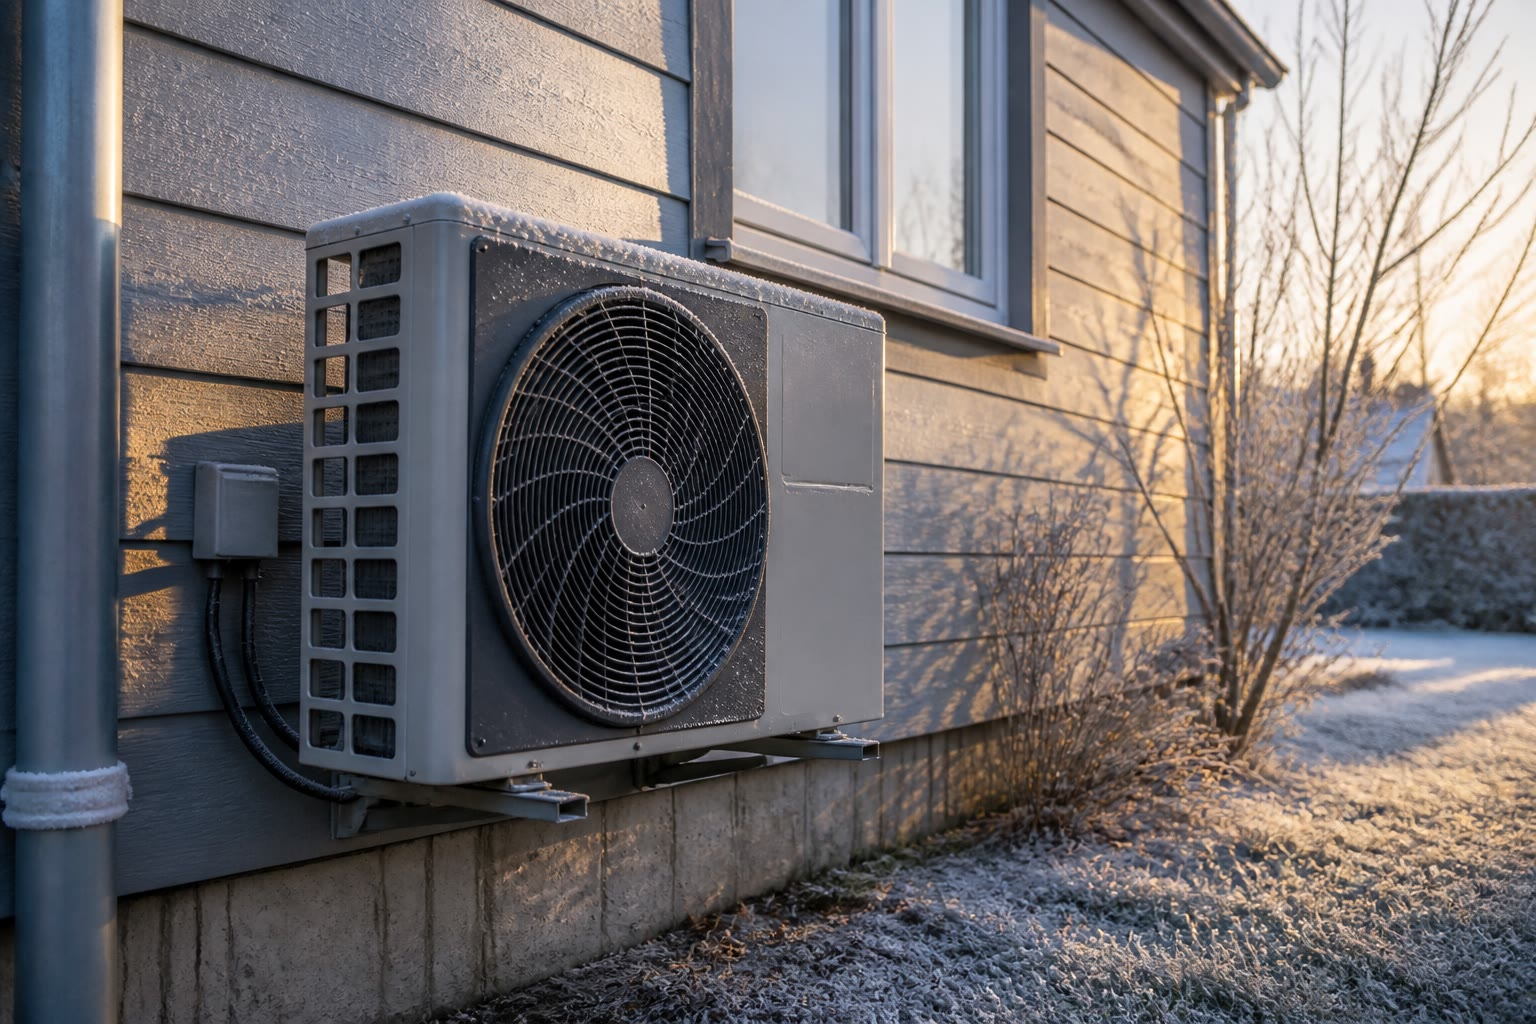
\includegraphics[width=0.58\linewidth]{images/book4/ai/b4-27-heat-pump-winter.jpg}

{\small The outdoor unit of a heat pump on a winter morning: a fan
draws cold air over the evaporator, and inside a compressor, a
condenser and a valve move that heat, three or four times multiplied,
into the house.}
\end{omfigure}

\section{Open systems and the mass balance}

\begin{definition}[Open system, control volume, steady flow]\label{def:b2:open-systems:cv}
An \emph{open system}\index{open system} is a fixed region of space,
the \emph{control volume}\index{control volume} $\Sigma$, bounded by a
surface through which fluid enters and leaves (inlet and outlet
sections) and through which heat and work can be exchanged with the
outside; the work received through moving parts (a shaft, a piston)
other than the flow itself is the \emph{useful work}\index{useful work}
$W_{\text{u}}$ (shaft work). The flow is \emph{steady}\index{steady
flow} when every field inside $\Sigma$ is time-independent: the mass,
energy and entropy contained in $\Sigma$ are then constant.
\end{definition}

\begin{proposition}[Mass balance]\label{prop:b2:open-systems:mass}
Through a section of area $S$ where the fluid of density $\rho$ moves
at the mean speed $c$ normal to it flows the \emph{mass flow
rate}\index{mass flow rate} $\dot m = \rho c S$ (in \unit{kg/s}). In a
\omterm{def:b2:open-systems:cv}{steady flow}, what enters leaves: $\sum_{\text{in}}\dot m = \sum_{\text{out}}
\dot m$; for a single stream, $\dot m$ is the same at inlet and outlet,
$\rho_1c_1S_1 = \rho_2c_2S_2$ --- the \omterm{thm:b2:fluid-kinematics:continuity}{continuity equation} of
\cref{ch:b2:fluid-kinematics} integrated over the section.
\end{proposition}

\begin{proof}
The mass in $\Sigma$ is constant, so the fluxes balance.
\end{proof}

\section{The first law for an open system}

\begin{theorem}[Energy balance of a steady single-stream flow]\label{thm:b2:open-systems:firstlaw}
For a \omterm{def:b2:open-systems:cv}{steady flow} of \omterm{def:b2:fluid-kinematics:flowrate}{mass flow rate} $\dot m$ entering at the state 1
and leaving at the state 2, receiving the useful (shaft) power
$P_{\text{u}}$ and the thermal power $P_{\text{th}}$,
\[
\dot m\,\Big[(h_2 - h_1) + \tfrac12(c_2^2 - c_1^2) + g(z_2 - z_1)\Big]
= P_{\text{u}} + P_{\text{th}} ,
\]
or, per unit mass of fluid crossing the system,
\[
\Delta h + \Delta\big(\tfrac12c^2\big) + g\,\Delta z = w_{\text{u}} + q .
\]
The \emph{enthalpy}\index{enthalpy (in a flow)} $h = u + Pv$ replaces
the internal energy: $Pv$ is the \emph{flow work}, the work done by
the upstream fluid to push a unit mass in, minus that done to push it
out.
\end{theorem}

\begin{proof}
Follow the closed system made of the fluid inside $\Sigma$ at $t$ plus
the slug $\dd m = \dot m\,\dd t$ about to enter; at $t + \dd t$ it
consists of the fluid inside $\Sigma$ (same state, \omterm{def:b2:open-systems:cv}{steady}) plus the
slug $\dd m$ that has left. Its energy changed by
$\dd m\,[(u_2 + \tfrac12c_2^2 + gz_2) - (u_1 + \tfrac12c_1^2 + gz_1)]$. It
received $P_{\text{u}}\dd t + P_{\text{th}}\dd t$, plus the work of the
pressure forces at the inlet, $P_1S_1 \times c_1\dd t = P_1v_1\,\dd m$
(pushing the slug in), minus that at the outlet, $P_2v_2\,\dd m$. The
first law for this closed system, with $u + Pv = h$, gives the result.
\end{proof}

\begin{omfigure}
\begin{tikzpicture}[scale=0.95, >=stealth]
  \draw[thick, rounded corners=6pt, fill=omDef!8] (1.2,0) rectangle (6.2,2.6);
  \node[font=\scriptsize] at (3.7,1.9) {control volume $\Sigma$ (steady)};
  % inlet pipe
  \draw[thick] (-0.6,0.5) -- (1.2,0.5); \draw[thick] (-0.6,1.1) -- (1.2,1.1);
  \fill[omExo!40] (-0.5,0.52) rectangle (0.1,1.08);
  \node[font=\scriptsize, above] at (-0.2,1.12) {$\dd m$};
  \draw[->, omExo, thick] (-1.4,0.8) -- (-0.6,0.8);
  \node[font=\scriptsize, left] at (-1.4,0.8) {$\dot m$, $h_1$, $c_1$, $z_1$};
  % outlet pipe
  \draw[thick] (6.2,1.5) -- (8.0,1.5); \draw[thick] (6.2,2.1) -- (8.0,2.1);
  \fill[omExo!40] (7.3,1.52) rectangle (7.9,2.08);
  \node[font=\scriptsize, above] at (7.6,2.12) {$\dd m$};
  \draw[->, omExo, thick] (8.0,1.8) -- (8.8,1.8);
  \node[font=\scriptsize, right] at (8.8,1.8) {$h_2$, $c_2$, $z_2$};
  % shaft
  \draw[->, omThm, very thick] (3.7,-0.8) -- (3.7,0) node[pos=0, below, font=\scriptsize] {$P_{\text{u}}$ (shaft)};
  \draw[->, omThm, very thick] (5.5,3.4) -- (5.5,2.6) node[pos=0, above, font=\scriptsize] {$P_{\text{th}}$};
  % pressure pushes
  \node[font=\scriptsize, omExo] at (0.3,0.2) {$P_1v_1$ pushes in};
  \node[font=\scriptsize, omExo] at (7.2,1.2) {$P_2v_2$ pushes out};
\end{tikzpicture}

{\small The \omterm{def:b2:open-systems:cv}{steady} \omterm{def:b2:open-systems:cv}{open system}: the closed system followed during $\dd
t$ is the contents of $\Sigma$ plus the entering slug, then the contents
plus the leaving slug; the pressure work at the two sections turns $u$
into $h = u + Pv$.}
\end{omfigure}

\begin{remark}[Using the first law]\label{rem:b2:open-systems:using}
For an ideal gas $\Delta h = c_p\Delta T$; for a liquid $\Delta h \approx
c\,\Delta T + v\,\Delta P$ (the second term is the pump's work); for a vapour
one reads $h$ from tables or charts. The kinetic term is usually
negligible: at \qty{10}{m/s}, $c^2/2 = \qty{50}{J/kg}$, against
\qty{1}{kJ/kg} for one kelvin of air --- it matters only in \omterm{prop:b2:open-systems:devices}{nozzles} and
turbine blades, where speeds reach hundreds of metres per second. The
potential term, $g\Delta z \approx \qty{10}{J/kg}$ per metre, matters for
water in a dam, never in a gas cycle. With several inlets and outlets
the balance reads $\sum_{\text{out}}\dot m\,h - \sum_{\text{in}}\dot m\,h =
P_{\text{u}} + P_{\text{th}}$ (kinetic and potential terms neglected).
\end{remark}

\section{The second law for an open system}

\begin{theorem}[Entropy balance of a steady flow]\label{thm:b2:open-systems:secondlaw}
For a \omterm{def:b2:open-systems:cv}{steady} single-stream flow exchanging the thermal powers
$P_{\text{th},i}$ with sources at the temperatures $T_i$,
\[
\dot m\,(s_2 - s_1) = \sum_i\frac{P_{\text{th},i}}{T_i} + \dot S_{\text{c}},
\qquad \dot S_{\text{c}} \ge 0 ;
\]
per unit mass, $\Delta s = s_{\text{exch}} + s_{\text{c}}$. An adiabatic
reversible flow is \emph{isentropic}; an adiabatic real flow has $s_2 >
s_1$. The \emph{isentropic efficiency}\index{isentropic efficiency} of
a turbine is $\eta_{\text{T}} = w_{\text{real}}/w_{\text{s}} = (h_1 - h_2)/(h_1
- h_{2s})$ and that of a compressor $\eta_{\text{C}} = (h_{2s} - h_1)/(h_2 -
h_1)$, where $2s$ is the state reached isentropically at the same
outlet pressure; both are typically $0.8$--$0.9$. The work lost to
irreversibility, referred to the ambient temperature $T_0$, is
$T_0\,s_{\text{c}}$ per unit mass.
\end{theorem}

\begin{proof}
Same closed system as before: its entropy changes by $\dd m\,(s_2 -
s_1)$, receives $\sum P_{\text{th},i}\dd t/T_i$ from the sources, and the
rest is created.
\end{proof}

\section{Elementary devices}

\begin{proposition}[Nozzle, throttle, compressor, turbine, exchanger]\label{prop:b2:open-systems:devices}
All adiabatic unless stated, \omterm{def:b2:open-systems:cv}{steady}, kinetic and potential terms
neglected unless they are the point.
\begin{itemize}
\item \emph{Nozzle}\index{nozzle} (no shaft, no heat): $\tfrac12c_2^2 -
      \tfrac12c_1^2 = h_1 - h_2$ --- \omterm{thm:b2:open-systems:firstlaw}{enthalpy} becomes speed; a
      \emph{diffuser} does the reverse.
\item \emph{Throttle}\index{throttle} (valve, porous plug; no shaft,
      no heat, speeds small): $h_2 = h_1$, \emph{isenthalpic}. For an
      ideal gas $T_2 = T_1$; for a real gas the temperature generally
      drops (Joule--Thomson effect); for a liquid near saturation a
      fraction flashes into vapour --- the expansion valve of every
      refrigerator.
\item \emph{Compressor, pump, turbine}\index{turbine} (adiabatic
      machines): $w_{\text{u}} = h_2 - h_1$ --- positive for a compressor,
      negative for a turbine; for a liquid pump $w_{\text{u}} \approx
      v(P_2 - P_1)$, tiny because $v$ is small.
\item \emph{Heat exchanger}\index{heat exchanger} (two streams, no
      shaft, adiabatic as a whole): $\dot m_{\text{a}}(h_{\text{a},2} -
      h_{\text{a},1}) = -\dot m_{\text{b}}(h_{\text{b},2} - h_{\text{b},1})$
      --- what one loses the other gains; the exchange creates entropy
      unless the streams are at the same temperature everywhere
      (counter-flow reduces it).
\item \emph{Mixing chamber}: $\sum\dot m_{\text{in}}h_{\text{in}} = \dot
      m_{\text{out}}h_{\text{out}}$.
\end{itemize}
\end{proposition}

\begin{proof}
Each is the first law with the appropriate terms set to zero.
\end{proof}

\begin{omfigure}
\begin{tikzpicture}[scale=0.85, >=stealth]
  % nozzle
  \draw[thick] (0,0.2) -- (1.6,0.55) -- (1.6,0.85) -- (0,1.2);
  \draw[->, omExo, thick] (-0.6,0.7) -- (-0.1,0.7);
  \draw[->, omExo, very thick] (1.7,0.7) -- (2.9,0.7);
  \node[font=\scriptsize] at (1.0,-0.35) {nozzle: $h \to c^2/2$};
  % throttle
  \begin{scope}[xshift=4.6cm]
    \draw[thick] (0,0.4) -- (1.0,0.4) -- (1.0,0.55) -- (1.2,0.55) -- (1.2,0.4) -- (2.4,0.4);
    \draw[thick] (0,1.0) -- (1.0,1.0) -- (1.0,0.85) -- (1.2,0.85) -- (1.2,1.0) -- (2.4,1.0);
    \draw[->, omExo, thick] (-0.6,0.7) -- (-0.1,0.7);
    \draw[->, omExo, thick] (2.5,0.7) -- (3.1,0.7);
    \node[font=\scriptsize] at (1.2,-0.35) {throttle: $h_2 = h_1$};
    \node[font=\scriptsize] at (0.4,1.3) {$P_1$}; \node[font=\scriptsize] at (2.0,1.3) {$P_2 < P_1$};
  \end{scope}
  % turbine
  \begin{scope}[xshift=9.6cm]
    \draw[thick] (0,1.3) -- (0,0.1) -- (2.0,-0.3) -- (2.0,1.7) -- cycle;
    \draw[->, omExo, thick] (-0.7,1.0) -- (-0.1,1.0);
    \draw[->, omExo, thick] (2.1,0.3) -- (2.8,0.3);
    \draw[->, omThm, very thick] (1.0,-0.4) -- (1.0,-1.0) node[below, font=\scriptsize] {$w_{\text{u}} = h_2 - h_1 < 0$};
    \node[font=\scriptsize] at (1.0,2.0) {turbine};
  \end{scope}
  % exchanger
  \begin{scope}[yshift=-3.2cm]
    \draw[thick, rounded corners=4pt] (0,0) rectangle (4.4,1.4);
    \draw[->, omExo, very thick] (-0.6,1.1) -- (0,1.1); \draw[omExo, very thick] (0,1.1) -- (4.4,1.1); \draw[->, omExo, very thick] (4.4,1.1) -- (5.0,1.1);
    \draw[<-, omDef, very thick] (-0.6,0.3) -- (0,0.3); \draw[omDef, very thick] (0,0.3) -- (4.4,0.3); \draw[<-, omDef, very thick] (4.4,0.3) -- (5.0,0.3);
    \node[font=\scriptsize, omExo, left] at (-0.6,1.1) {hot in}; \node[font=\scriptsize, omExo, right] at (5.0,1.1) {hot out};
    \node[font=\scriptsize, omDef, right] at (5.0,0.3) {cold in}; \node[font=\scriptsize, omDef, left] at (-0.6,0.3) {cold out};
    \node[font=\scriptsize] at (2.2,-0.4) {counter-flow exchanger: $\dot m_{\text{a}}\Delta h_{\text{a}} = -\dot m_{\text{b}}\Delta h_{\text{b}}$};
    \node[font=\scriptsize] at (8.4,0.7) {(the mixing chamber: $\sum\dot m_{\text{in}}h_{\text{in}} = \dot m_{\text{out}}h_{\text{out}}$)};
  \end{scope}
\end{tikzpicture}

{\small The elementary \omterm{def:b2:open-systems:cv}{open systems}: each is the energy balance with
the irrelevant terms struck out --- no shaft in a \omterm{prop:b2:open-systems:devices}{nozzle} or a \omterm{prop:b2:open-systems:devices}{throttle},
no heat in an adiabatic turbine, no net heat for an exchanger taken as
a whole.}
\end{omfigure}

\begin{example}[Numbers for the devices]\label{ex:b2:open-systems:numbers}
Steam entering a turbine \omterm{prop:b2:open-systems:devices}{nozzle} at $h = \qty{3000}{kJ/kg}$ and leaving
at \qty{2800}{kJ/kg} reaches $c = \sqrt{2 \times 200 \times 10^3} =
\qty{630}{m/s}$. Air compressed adiabatically from \qty{1}{bar},
\qty{293}{K} to \qty{8}{bar}: isentropically $T_2 = 293 \times 8^{0.286} =
\qty{531}{K}$ and $w = c_p\Delta T = \qty{239}{kJ/kg}$; with $\eta_{\text{C}} =
0.8$, \qty{299}{kJ/kg} and \qty{590}{K} --- which is why compressors are
cooled between stages. A car radiator removing \qty{42}{kW} from water
cooled by \qty{10}{K} (\qty{1}{kg/s}) warms \qty{2.1}{kg/s} of air by
\qty{20}{K}. Liquid refrigerant at \qty{40}{\celsius} throttled to
\qty{0}{\celsius} arrives as a mist with $28\%$ of vapour: the flashing
is what cools the liquid to the evaporator temperature.
\end{example}

\section{Cycles}

\begin{proposition}[Vapour-compression refrigeration and heat pump]\label{prop:b2:open-systems:fridge}
A refrigerant circulates through: (1$\to$2) an adiabatic compressor
that raises the vapour from the evaporator pressure to the condenser
pressure, $w = h_2 - h_1$; (2$\to$3) a condenser where it releases
$q_{\text{cond}} = h_2 - h_3$ to the hot side (the room for a heat pump, the
kitchen for a fridge) and leaves as a liquid; (3$\to$4) a \omterm{prop:b2:open-systems:devices}{throttle}, $h_4
= h_3$; (4$\to$1) an evaporator where it absorbs $q_{\text{evap}} = h_1 - h_4$
from the cold side. The coefficients of performance are
\[
\mathrm{COP}_{\text{cooling}} = \frac{h_1 - h_4}{h_2 - h_1}, \qquad
\mathrm{COP}_{\text{heating}} = \frac{h_2 - h_3}{h_2 - h_1} = \mathrm{COP}_{\text{cooling}} + 1 ,
\]
bounded by Carnot's $T_{\text{c}}/(T_{\text{h}} - T_{\text{c}})$ and
$T_{\text{h}}/(T_{\text{h}} - T_{\text{c}})$; the cycle is read most easily on
the $(\log P, h)$ diagram, where the two exchanges and the work are
horizontal segments.
\end{proposition}

\begin{proof}
The four first-law balances; the energy balance of the whole cycle
gives $q_{\text{cond}} = q_{\text{evap}} + w$, hence the relation between
the two COPs.
\end{proof}

\begin{omfigure}
\begin{tikzpicture}
  \begin{axis}[width=8.6cm, height=5.2cm, xmin=150, xmax=480, ymin=-0.1, ymax=1.5,
    axis x line=bottom, axis y line=left, xlabel={$h$ (\unit{kJ/kg})}, ylabel={$\log P$},
    xlabel style={at={(axis description cs:0.5,-0.12)}, anchor=north}, ytick=\empty, xtick={200,300,400}, clip=false]
    % saturation dome (schematic)
    \addplot[gray, thick, smooth] coordinates {(200,0.3) (215,0.55) (232,0.85) (256,1.1) (290,1.3) (330,1.38) (370,1.3) (405,1.1) (418,0.85) (418,0.55) (399,0.3)};
    % cycle
    \draw[omDef, very thick] (axis cs:256,1.1) -- (axis cs:256,0.3);
    \draw[omDef, very thick] (axis cs:256,0.3) -- (axis cs:399,0.3);
    \draw[omDef, very thick] (axis cs:399,0.3) -- (axis cs:433,1.1);
    \draw[omDef, very thick] (axis cs:433,1.1) -- (axis cs:256,1.1);
    \fill (axis cs:399,0.3) circle (1.5pt) node[below, font=\scriptsize] {1};
    \fill (axis cs:433,1.1) circle (1.5pt) node[above, font=\scriptsize] {2};
    \fill (axis cs:256,1.1) circle (1.5pt) node[above, font=\scriptsize] {3};
    \fill (axis cs:256,0.3) circle (1.5pt) node[below, font=\scriptsize] {4};
    \node[font=\scriptsize, omDef] at (axis cs:330,0.2) {evaporator $q_{\text{evap}}$};
    \node[font=\scriptsize, omDef] at (axis cs:345,1.2) {condenser $q_{\text{cond}}$};
    \node[font=\scriptsize, omDef, anchor=west] at (axis cs:418,0.68) {$w$};
    \node[font=\scriptsize, gray] at (axis cs:205,0.95) {liquid};
    \node[font=\scriptsize, gray] at (axis cs:450,0.5) {vapour};
    \node[font=\scriptsize, gray] at (axis cs:330,0.75) {liquid + vapour};
  \end{axis}
\end{tikzpicture}

{\small The vapour-compression cycle on the $(\log P, h)$ chart: the
condenser and evaporator are isobars inside the dome, the \omterm{prop:b2:open-systems:devices}{throttle} a
vertical isenthalp, the compressor a slanted line; the lengths of the
horizontal segments are the heats and the work per kilogram.}
\end{omfigure}

\begin{proposition}[The steam (Rankine) cycle]\label{prop:b2:open-systems:rankine}
Water circulates through: (1$\to$2) a pump, $w_{\text{p}} \approx v(P_2 -
P_1)$, a few \unit{kJ/kg}; (2$\to$3) a boiler at high pressure where it
is heated, vaporised and superheated, $q_{\text{in}} = h_3 - h_2$;
(3$\to$4) a turbine expanding the steam to the condenser pressure,
$w_{\text{t}} = h_3 - h_4$ (a thousand \unit{kJ/kg}); (4$\to$1) a condenser
at low pressure where the wet steam turns back to liquid, rejecting
$q_{\text{out}} = h_4 - h_1$ to the cooling water. The efficiency is
\[
\eta = \frac{w_{\text{t}} - w_{\text{p}}}{q_{\text{in}}} = 1 - \frac{q_{\text{out}}}{q_{\text{in}}} ,
\]
about $0.35$--$0.45$ in practice; the heat is added at a mean
temperature $\bar T = q_{\text{in}}/(s_3 - s_2)$ well below the boiler's
peak, which is why superheating, reheating and high pressures raise
$\eta$, and why the exhaust must stay dry enough ($x_4 \gtrsim 0.88$) to
spare the last blades from droplet erosion.
\end{proposition}

\begin{proof}
First law on each component, then on the cycle: $w_{\text{t}} - w_{\text{p}}
= q_{\text{in}} - q_{\text{out}}$.
\end{proof}

\begin{omfigure}
\begin{tikzpicture}
  \begin{axis}[width=8.4cm, height=5.2cm, xmin=0, xmax=9.5, ymin=250, ymax=820,
    axis x line=bottom, axis y line=left, xlabel={$s$ (\unit{kJ/kg/K})}, ylabel={$T$ (\unit{K})},
    xlabel style={at={(axis description cs:0.5,-0.12)}, anchor=north}, xtick={2,4,6,8}, ytick={300,500,700}, clip=false]
    % dome
    \addplot[gray, thick, smooth] coordinates {(0.4,280) (1.3,373) (2.3,473) (3.3,560) (4.4,647) (5.5,600) (6.3,520) (7.1,440) (7.9,373) (8.4,306)};
    % cycle: 1 (0.48,306) 2 (0.5,308) along sat liquid to 549K (3.1,549) then vaporise to (5.9,549) then superheat to 3 (6.88,773); expand to 4 (7.53,306); back to 1
    \draw[omDef, very thick] (axis cs:0.48,306) -- (axis cs:0.5,309);
    \draw[omDef, very thick, smooth] plot coordinates {(0.5,309) (1.2,373) (2.2,470) (3.1,549)};
    \draw[omDef, very thick] (axis cs:3.1,549) -- (axis cs:5.9,549);
    \draw[omDef, very thick, smooth] plot coordinates {(5.9,549) (6.3,620) (6.88,773)};
    \draw[omDef, very thick] (axis cs:6.88,773) -- (axis cs:7.53,306);
    \draw[omDef, very thick, dashed] (axis cs:6.88,773) -- (axis cs:6.88,306);
    \draw[omDef, very thick] (axis cs:7.53,306) -- (axis cs:0.48,306);
    \fill (axis cs:0.48,306) circle (1.5pt) node[below left, font=\scriptsize] {1,2};
    \fill (axis cs:6.88,773) circle (1.5pt) node[above, font=\scriptsize] {3};
    \fill (axis cs:7.53,306) circle (1.5pt) node[below, font=\scriptsize] {4};
    \fill (axis cs:6.88,306) circle (1.5pt) node[below, font=\scriptsize] {4s};
    \node[font=\scriptsize, omDef] at (axis cs:3.8,600) {boiler};
    \node[font=\scriptsize, omDef, anchor=west] at (axis cs:7.3,560) {turbine};
    \node[font=\scriptsize, omDef] at (axis cs:4.0,285) {condenser};
  \end{axis}
\end{tikzpicture}

{\small The Rankine cycle on the $(T,s)$ diagram: pump (invisible),
heating along the liquid line, vaporisation at the boiler pressure,
superheat, expansion (isentropic dashed, real solid, ending wetter or
drier), condensation. The mean temperature of heat addition, not the
peak, sets the efficiency.}
\end{omfigure}

\begin{remark}[Other cycles, and a transient]\label{rem:b2:open-systems:other}
The gas turbine (compressor, combustion chamber, turbine: the Brayton
cycle) has the ideal efficiency $1 - r^{-(\gamma-1)/\gamma}$ for the
pressure ratio $r$ and rejects its exhaust at several hundred degrees;
feeding that exhaust to a steam cycle (combined cycle) reaches $60\%$.
\omterm{def:b2:open-systems:cv}{Open systems} also have transients: filling an evacuated rigid tank from
a line at $T_0$ ends at $T = \gamma T_0$ (the flow work $Pv$ becomes
internal energy), \qty{120}{K} hotter for air --- the reason a diving
bottle warms as it is filled.
\end{remark}

\begin{method}[Open-system balances]\label{meth:b2:open-systems:method}
(1) Draw the \omterm{def:b2:open-systems:cv}{control volume}; list inlets, outlets, shaft and heat.
(2) Mass: $\sum\dot m_{\text{in}} = \sum\dot m_{\text{out}}$. (3) Energy
per unit mass: $\Delta h + \Delta c^2/2 + g\Delta z = w_{\text{u}} + q$, with
$\Delta h = c_p\Delta T$ for gases, tables for vapours, $v\Delta P$ for
pumps. (4) Entropy: $\Delta s = \sum q_i/T_i + s_{\text{c}}$, isentropic
reference states, efficiencies, $T_0s_{\text{c}}$ lost. (5) Cycles: read
the chart, sum around the loop, compare with Carnot.
\end{method}

\section{Exercises}

\begin{exercise}[$\star$]\label{exo:b2:open-systems:1}
(a) A garden hose delivers \qty{12}{L/min} through a \qty{1}{cm}
\omterm{prop:b2:open-systems:devices}{nozzle}: exit speed. (b) Hot water at \qty{60}{\celsius}, \qty{0.1}{kg/s},
mixes with cold water at \qty{10}{\celsius}, \qty{0.2}{kg/s}: outlet
temperature. (c) Why is the mixing irreversible --- compute the
entropy created per second.
\end{exercise}

\begin{exercise}[$\star$]\label{exo:b2:open-systems:2}
Steam enters a \omterm{prop:b2:open-systems:devices}{nozzle} at \qty{50}{m/s} with $h = \qty{3000}{kJ/kg}$ and
leaves with \qty{2800}{kJ/kg}: exit speed. Air at \qty{300}{K} accelerated
from rest to \qty{300}{m/s} in a \omterm{prop:b2:open-systems:devices}{nozzle} ($c_p = \qty{1005}{J/kg/K}$):
temperature drop. A diffuser slows air from \qty{250}{m/s} to rest: rise.
\end{exercise}

\begin{exercise}[$\star$]\label{exo:b2:open-systems:3}
Throttling. (a) An ideal gas: what happens to $T$, to $s$? (b) Wet steam
at \qty{10}{bar} ($h_{\text{f}} = 763$, $h_{\text{fg}} = \qty{2015}{kJ/kg}$),
quality $0.9$, throttled to \qty{1}{bar} ($h_{\text{f}} = 417$, $h_{\text{fg}}
= \qty{2258}{kJ/kg}$): final quality --- the throttling calorimeter. (c)
Liquid refrigerant at \qty{40}{\celsius} ($h = \qty{256}{kJ/kg}$) throttled
to \qty{0}{\celsius} ($h_{\text{f}} = 200$, $h_{\text{g}} = \qty{399}{kJ/kg}$):
vapour fraction.
\end{exercise}

\begin{exercise}[$\star$]\label{exo:b2:open-systems:4}
(a) A radiator cools \qty{1}{kg/s} of water from \qty{90}{} to \qty{80}{\celsius};
the air ($c_p = \qty{1005}{J/kg/K}$) warms from \qty{20}{} to \qty{40}{\celsius}:
air mass flow and volume flow. (b) A steam turbine, \qty{10}{kg/s},
$h$ from \qty{3400}{} to \qty{2400}{kJ/kg}: power. (c) A pump raises
water from \qty{1}{} to \qty{60}{bar}: work per kilogram, and power for
\qty{500}{kg/s}.
\end{exercise}

\begin{exercise}[$\star\star$]\label{exo:b2:open-systems:5}
\emph{The flow work.} (a) Re-derive the open-system first law and
explain where $Pv$ comes from. (b) Why does the internal energy $u$
appear in a closed system and $h$ in a flow? (c) Compare $c^2/2$ at
\qty{10}{m/s} and \qty{300}{m/s} with $c_p\Delta T$ for \qty{1}{K} of air.
(d) Water falling \qty{100}{m} through a penstock: $g\Delta z$ against
$c\,\Delta T$ for \qty{1}{K}; conclude how much the water warms if the
turbine is removed.
\end{exercise}

\begin{exercise}[$\star\star$]\label{exo:b2:open-systems:6}
\emph{Compressors.} Air, \qty{1}{bar}, \qty{293}{K}, to \qty{8}{bar}; $\gamma =
1.4$, $c_p = \qty{1005}{J/kg/K}$, $r = \qty{287}{J/kg/K}$. (a) Isentropic
outlet temperature and work. (b) With $\eta_{\text{C}} = 0.8$: work, outlet
temperature, entropy created. (c) Two stages of ratio $\sqrt8$ with
cooling back to \qty{293}{K} between them: work saved. (d) Isothermal
limit $rT\ln 8$; why real compressors approach it with many stages.
\end{exercise}

\begin{exercise}[$\star\star$]\label{exo:b2:open-systems:7}
\emph{Turbine.} Steam at \qty{60}{bar}, \qty{500}{\celsius}: $h_3 = \qty{3422}{kJ/kg}$,
$s_3 = \qty{6.88}{kJ/kg/K}$; condenser \qty{0.05}{bar} (\qty{33}{\celsius}):
$s_{\text{f}} = 0.476$, $s_{\text{g}} = \qty{8.394}{kJ/kg/K}$, $h_{\text{f}} = 138$,
$h_{\text{fg}} = \qty{2423}{kJ/kg}$. (a) Isentropic exit quality and
\omterm{thm:b2:open-systems:firstlaw}{enthalpy}, work. (b) With $\eta_{\text{T}} = 0.85$: work, exit \omterm{thm:b2:open-systems:firstlaw}{enthalpy} and
quality. (c) Entropy created per kilogram and lost work at $T_0 =
\qty{306}{K}$. (d) Why a too-wet exhaust is a problem.
\end{exercise}

\begin{exercise}[$\star\star$]\label{exo:b2:open-systems:8}
\emph{Heat pump.} Evaporator \qty{0}{\celsius}, condenser \qty{40}{\celsius};
$h_1 = 399$ (saturated vapour, \qty{0}{\celsius}), $h_{2s} = 426$, $h_3 = 256$,
$h_4 = h_3$ (\unit{kJ/kg}); $\eta_{\text{C}} = 0.8$. (a) $h_2$ and the work.
(b) Heats exchanged, both COPs. (c) Carnot COPs; ratio. (d) Mass flow
and electrical power for \qty{8}{kW} of heating; why the COP falls when
the outdoor air gets colder.
\end{exercise}

\begin{exercise}[$\star\star$]\label{exo:b2:open-systems:9}
\emph{Entropy in an exchanger.} Hot water \qty{1}{kg/s} from \qty{90}{} to
\qty{50}{\celsius} heats cold water \qty{2}{kg/s} from \qty{10}{\celsius}.
(a) Outlet temperature of the cold stream. (b) Entropy created per
second ($c = \qty{4180}{J/kg/K}$). (c) Lost power at $T_0 = \qty{293}{K}$,
compared with the \qty{167}{kW} exchanged. (d) Why would a parallel-flow
arrangement create more entropy than counter-flow for the same duty?
\end{exercise}

\begin{exercise}[$\star\star\star$]\label{exo:b2:open-systems:10}
\emph{Filling a tank.} A rigid, evacuated, insulated tank is connected
to a line carrying an ideal gas at $T_0$, $P_0$. (a) Write the energy
balance of the tank during filling (unsteady: its energy grows) and
show that the gas inside ends at $T = \gamma T_0$. (b) Air at \qty{293}{K}:
final temperature. (c) If the tank initially held gas at $T_0$ and
$P_1 < P_0$, argue that the final temperature lies between $T_0$ and
$\gamma T_0$. (d) Why does a scuba bottle warm when filled, and why is
it filled slowly in water?
\end{exercise}

\begin{exercise}[$\star\star\star$]\label{exo:b2:open-systems:11}
\emph{Reheat.} The turbine of \cref{exo:b2:open-systems:7} is split:
expansion to \qty{10}{bar} (isentropic end: $h = \qty{2850}{kJ/kg}$), reheat
to \qty{500}{\celsius} ($h = 3478$, $s = \qty{7.76}{kJ/kg/K}$), expansion to
\qty{0.05}{bar}, both stages isentropic. Pump work \qty{6}{kJ/kg}, $h_2 =
\qty{144}{kJ/kg}$. (a) Exit quality and \omterm{thm:b2:open-systems:firstlaw}{enthalpy} of the second stage. (b)
Total work and heat; efficiency; compare with the single expansion
($\eta = 0.40$ isentropic). (c) Why does reheat help, in terms of the
mean temperature of heat addition? (d) What else does it fix?
\end{exercise}

\begin{exercise}[$\star\star\star$]\label{exo:b2:open-systems:12}
\emph{Gas turbine and combined cycle.} Air compressed isentropically
from \qty{1}{bar}, \qty{293}{K} to \qty{12}{bar}, heated at constant pressure
to \qty{1500}{K}, expanded isentropically to \qty{1}{bar}; $\gamma = 1.4$,
$c_p = \qty{1005}{J/kg/K}$. (a) The four temperatures. (b) Works,
heat, efficiency; show $\eta = 1 - r^{-(\gamma - 1)/\gamma}$. (c) The
exhaust at $T_4$ raises steam for a Rankine cycle of efficiency $0.35$
that recovers $70\%$ of the exhaust's heat above \qty{373}{K}: combined
efficiency. (d) Why is the combined cycle the most efficient thermal
plant there is?
\end{exercise}

\section{Problem: A domestic heat pump and a steam power plant}

\begin{problem}[{Weekend problem --- two machines sized with the
open-system balances}]\label{pb:b2:open-systems:1}
\textbf{Part I --- The heat pump.}
Refrigerant data (\unit{kJ/kg}, \unit{kJ/kg/K}): saturated vapour at
\qty{0}{\celsius} ($P = \qty{2.9}{bar}$): $h_1 = 399$, $s_1 = 1.727$;
saturated liquid at \qty{0}{\celsius}: $h_{\text{f}} = 200$, $s_{\text{f}} = 1.00$;
at the condenser pressure \qty{10.2}{bar} ($T_{\text{sat}} = \qty{40}{\celsius}$):
isentropic compression end $h_{2s} = 426$, saturated liquid $h_3 = 256$,
$s_3 = 1.19$; superheated vapour there has $c_p \approx \qty{1.0}{kJ/kg/K}$.
Compressor $\eta_{\text{C}} = 0.8$; house demand \qty{8}{kW}.
\begin{enumerate}
  \item Sketch the cycle on a $(\log P, h)$ chart and name the four
        components with the process each performs.
  \item State 4 after the \omterm{prop:b2:open-systems:devices}{throttle}: \omterm{thm:b2:open-systems:firstlaw}{enthalpy} and vapour fraction.
  \item Heat absorbed per kilogram in the evaporator.
  \item Compressor work, isentropic and real; $h_2$ and an estimate of
        $T_2$.
  \item Heat released in the condenser; both COPs; check their
        relation.
  \item Carnot COPs between \qty{0}{} and \qty{40}{\celsius}; what
        fraction does the machine reach?
  \item Mass flow of refrigerant and electrical power (motor
        efficiency $0.9$).
  \item Entropy created per kilogram in the compressor and in the
        \omterm{prop:b2:open-systems:devices}{throttle} ($s_4 = s_{\text{f}} + x\,(s_1 - s_{\text{f}})$); which is
        worse?
\end{enumerate}

\textbf{Part II --- Cold weather and design choices.}
\begin{enumerate}[resume]
  \item At \qty{-10}{\celsius} outside the evaporator runs at
        \qty{-15}{\celsius}: Carnot COP for heating; why does the real
        COP fall faster (think of the pressure ratio and of the
        vapour's density)?
  \item Why does frost form on the outdoor coil, and what does the
        defrost cycle cost?
  \item Underfloor heating at \qty{35}{\celsius} versus radiators at
        \qty{55}{\celsius}: Carnot COPs with the evaporator at
        \qty{0}{\celsius}; conclude.
  \item Compare, per kilowatt-hour of fuel burnt in a power plant of
        efficiency $0.40$, the heat delivered by this heat pump ($\mathrm{COP}
        = 4$) and by a gas boiler of efficiency $0.9$ burning the fuel
        directly.
\end{enumerate}

\textbf{Part III --- The steam plant.}
Boiler \qty{60}{bar}, \qty{500}{\celsius}: $h_3 = 3422$, $s_3 = 6.88$; at
\qty{60}{bar}, $T_{\text{sat}} = \qty{276}{\celsius}$, $h_{\text{f}} = 1213$,
$h_{\text{g}} = 2784$; condenser \qty{0.05}{bar}, \qty{33}{\celsius}:
$h_{\text{f}} = 138$, $h_{\text{fg}} = 2423$, $s_{\text{f}} = 0.476$, $s_{\text{g}} =
8.394$; liquid $v = \qty{1e-3}{m^3/kg}$; turbine $\eta_{\text{T}} = 0.85$;
net electrical output \qty{600}{MW}.
\begin{enumerate}[resume]
  \item Sketch the cycle on a $(T,s)$ diagram and name the processes.
  \item Pump work and $h_2$.
  \item Heat added in the boiler, split into preheating, vaporisation
        and superheating.
  \item Isentropic expansion: exit quality, \omterm{thm:b2:open-systems:firstlaw}{enthalpy}, work.
  \item Real expansion: work, exit \omterm{thm:b2:open-systems:firstlaw}{enthalpy} and quality; why the
        quality matters.
  \item Cycle efficiency; Carnot between \qty{773}{} and \qty{306}{K};
        the mean temperature of heat addition $\bar T = q_{\text{in}}/(s_3
        - s_2)$ and the Carnot efficiency it would give.
  \item Steam mass flow; heat rejected in the condenser; cooling water
        flow for a \qty{10}{K} rise, or the mass of water a cooling
        tower evaporates per second (\qty{2.4}{MJ/kg}).
  \item Entropy created in the turbine per kilogram and per second;
        the work lost at \qty{306}{K}, as a fraction of the turbine
        work.
  \item Reheating at \qty{10}{bar} to \qty{500}{\celsius} raises the
        efficiency to about $0.43$ and the exit quality to $0.92$:
        explain both effects qualitatively.
\end{enumerate}

\textbf{Part IV --- The whole chain.}
\begin{enumerate}[resume]
  \item The furnace transfers its heat to the steam from flue gases at
        about \qty{1500}{K}: entropy created per second in that transfer
        (heat at \qty{1500}{K} into steam at $\bar T$); compare with the
        turbine's.
  \item The condenser rejects its heat to water at \qty{306}{K} ---
        which finally reaches the environment at \qty{293}{K}: entropy
        created per second there.
  \item Rank the three sources of irreversibility (furnace, turbine,
        condenser) and say where the engineers' effort goes.
  \item Summarise the open-system method in five lines.
\end{enumerate}
\end{problem}
